%%%%%%%%%%%%%%%%%%%%%%% file template.tex %%%%%%%%%%%%%%%%%%%%%%%%%
%
% This is a general template file for the LaTeX package SVJour3
% for Springer journals.          Springer Heidelberg 2010/09/16
%
% Copy it to a new file with a new name and use it as the basis
% for your article. Delete % signs as needed.
%
% This template includes a few options for different layouts and
% content for various journals. Please consult a previous issue of
% your journal as needed.
%
%%%%%%%%%%%%%%%%%%%%%%%%%%%%%%%%%%%%%%%%%%%%%%%%%%%%%%%%%%%%%%%%%%%
%
% First comes an example EPS file -- just ignore it and
% proceed on the \documentclass line
% your LaTeX will extract the file if required
%\begin{filecontents*}{example.eps}
%%!PS-Adobe-3.0 EPSF-3.0
%%%BoundingBox: 19 19 221 221
%%%CreationDate: Mon Sep 29 1997
%%%Creator: programmed by hand (JK)
%%%EndComments
%gsave
%newpath
%  20 20 moveto
%  20 220 lineto
%  220 220 lineto
%  220 20 lineto
%closepath
%2 setlinewidth
%gsave
%  .4 setgray fill
%grestore
%stroke
%grestore
%\end{filecontents*}
%
\RequirePackage{fix-cm}
%
%\documentclass{svjour3}                     % onecolumn (standard format)
%\documentclass[smallcondensed]{svjour3}     % onecolumn (ditto)
\documentclass[smallextended]{svjour3}       % onecolumn (second format)
%\documentclass[twocolumn]{svjour3}          % twocolumn
%
\smartqed  % flush right qed marks, e.g. at end of proof
%
\usepackage{soul}
\usepackage{bm,textcomp}

\usepackage{graphicx}
\usepackage{color}
\usepackage{natbib}
%
% \usepackage{mathptmx}      % use Times fonts if available on your TeX system
%
% insert here the call for the packages your document requires
%\usepackage{latexsym}
% etc.
%
% please place your own definitions here and don't use \def but
% \newcommand{}{}
%
% Insert the name of "your journal" with
\journalname{Journal of Membrane Biology}
%
\newcommand{\knw}[1]{\textcolor{blue}{KW: #1}}
\newcommand{\grace}[1]{\textcolor{blue}{GB: #1}}
\newcommand{\liam}[1]{\textcolor{red}{LM: #1}}


%%example: \kwn{sup}

\newcommand{\bemb}{n_{\mathrm{emb}}}
\newcommand{\bann}{n_{\mathrm{ann}}}
\newcommand{\femb}{f_{\mathrm{emb}}}
\newcommand{\fann}{f_{\mathrm{ann}}}
\newcommand{\qsat}{Q_{\mathrm{sat}}}
\newcommand{\qpufa}{Q_{\mathrm{DHA}}}
\newcommand{\xsat}{x_{\mathrm{sat}}}
\newcommand{\xch}{x_{\mathrm{Chol}}}
\newcommand{\nbound}{b_{\mathrm{tot}}}

\begin{document}

\title{Untangling direct and domain-mediated interactions between nicotinic acetylcholine receptors in DHA-rich membranes}
%\thanks{Grants or other notes
%about the article that should go on the front page should be
%placed here. General acknowledgments should be placed at the end of the article.}
%\subtitle{Do you have a subtitle?\\ If so, write it here}

%\titlerunning{Short form of title}        % if too long for running head

\author{Kristen Woods*         \and
        Liam Sharp* \and 
        Grace Brannigan$^\dagger$ %etc.
}

%\authorrunning{Short form of author list} % if too long for running head

\institute{Kristen Woods and Liam Sharp and Grace Brannigan \at
              Center for Computational and Integrative Biology, Rutgers University-Camden, Camden, NJ \\
              %Tel.: +123-45-678910\\
              %Fax: +123-45-678910\\
              %\email{fauthor@example.com}           %  \\
%             \emph{Present address:} of F. Author  %  if needed
           \and
         Grace Brannigan \at
             Department of Physics, Rutgers University-Camden, Camden, NJ
             \and
             *These authors contributed equally.  
            $^\dagger$Corresponding Author (grace.brannigan@rutgers.edu) 
}

\date{Received: date / Accepted: date}
% The correct dates will be entered by the editor
\titlerunning{Interactions among nAChRs in DHA-rich membranes}

\maketitle
\begin{abstract}

%Lipid composition of the membrane can strongly modulate both function and organization of the nicotinic acetylcholine receptor (nAChR). Previously we conducted coarse-grained molecular simulations of a single nAChR from the electric ray {\it torpedo} in mixed membranes, and observed that lipids containing long chain polyunsaturated fatty acids (PUFAs) like docosahexaenoic acid (DHA) were abundant among nAChR boundary lipids.   Using a similar approach to investigate the role of lipid topology and lipid domain formation, here
%At the neuromuscular junction, the nicotinic acetylcholine receptor (nAChR) self-associates to give rise to rapid muscle movement. While lipid domains have maintained nAChR aggregates in-vitro, their specific roles in nAChR clustering are currently unknown. In the present study, we carried out coarse-grained molecular dynamics simulations (CG-MD) of 1-4 nAChR molecules in two membrane environments: One mixture containing domain-forming, homoacidic lipids, and a second mixture consisting of heteroacidic lipids. Spontaneous dimerization of nAChRs was up to ten times more likely in domain-forming membranes; however, the effect was not significant in four-protein systems, suggesting that lipid domains are less critical to nAChR oligomerization when protein concentration is higher. With regard to lipid preferences, nAChRs consistently partitioned into liquid-disordered domains occupied by the omega-3 fatty acid, Docosahexaenoic acid (DHA); enrichment of DHA boundary lipids increased with protein concentration, particularly in homoacidic membranes. This result suggests dimer formation blocks access of saturated chains and cholesterol, but not polyunsaturated chains, to boundary lipid sites.
 
 
  
 
 
 
 
 
 At the neuromuscular junction (NMJ), the nicotinic acetylcholine receptor (nAChR) self-associates to give rise to rapid muscle movement. While lipid domains have maintained nAChR aggregates in-vitro, their specific roles in nAChR clustering are currently unknown. In the present study, we carried out coarse-grained molecular dynamics simulations (CG-MD) of 1-4 nAChR molecules in two membrane environments: One mixture containing domain-forming, homoacidic lipids, and a second mixture consisting of heteroacidic lipids. Spontaneous dimerization of nAChRs was up to ten times more likely in domain-forming membranes; however, the effect was not significant in four-protein systems, suggesting that lipid domains are less critical to nAChR oligomerization when protein concentration is higher. With regard to lipid preferences, nAChRs consistently partitioned into liquid-disordered domains occupied by the omega-3 ($\omega$-3) fatty acid, Docosahexaenoic acid (DHA); enrichment of DHA boundary lipids increased with protein concentration, particularly in homoacidic membranes. This result suggests dimer formation blocks access of saturated chains and cholesterol, but not polyunsaturated chains, to boundary lipid sites.   

%{ The nicotinic acetylcholine receptors (nAChR) are highly lipid sensitive pentameric ligand gated ion channels that agrigate into dense clusters, hypothesized to be driven by domain formation. We showed previously using coarse grained simulations\citep{Sharp2019} the nAChR domain partitioning, as well as annular and non-annular lipid interaction, are highly regulated by polyunsaturated fatty acids (PUFAs). Here, using coarse grained molecular dynamics, we investigated multiple replicas of membranes with one to four embedded nAChRs to try and resolve the effect of naChR clustering due to quasi-native membrane composition. All simulations had constant ratios of saturated fatty acids, PUFAs, and cholesterol; however domain forming membranes used lipids with homoacids (three lipid species), while non-domain forming membranes used lipids heteroacids (two lipid species). Results  show variation between both domain forming and non-domain forming membranes and thier lipids direct interaction with nAChR. More interestingly differences in direct interactions between lipids and one or more proteins are observed.  Specifically we see changes in annular lipids and embedded lipids distributions, distances between nAChR-nAChR pairs, and nAChR subunit-nAChR subunit interactions.}


\keywords{Nicotinic acetylcholine receptor (nAChR) \and Polyunsaturated fatty acids (PUFAs) \and Domain formation \and Lipid-protein interactions \and Lipid rafts \and Docosahexaenoic acid (DHA)}
% \PACS{PACS code1 \and PACS code2 \and more}
% \subclass{MSC code1 \and MSC code2 \and more}
\end{abstract}

\section{Introduction}
\label{intro}
%Your text comes here. Separate text sections with
%\subsection{Neuromuscular nicotinic acetylcholine receptors (nAChRs) and their lipid interactions}
%\label{sec:1}
The muscle-derived nicotinic acetylcholine receptor (nAChR) (PDB 2BG9) \citep{Unwin2005} is the most abundant neurotransmitter receptor at the neuromuscular junction (NMJ) in most vertebrates, including humans \citep{Albuquerque2009}. Within the postsynaptic membrane, nAChRs cluster in high densities (10,000 per $\mu$m$^{2}$) to properly activate the skeletal muscle \citep{Ramarao1998,Breckenridge1972}. As a major transmembrane protein, nAChR depends upon a highly specific lipid environment to maintain functionality. Lipids influence nAChR activity by affecting both function and organization. It is essential to understand how changes in lipid environment impact nAChR's structure and activity, given that lipids can change in response to aging and disease  \citep{Yadav2014}, and also vary across tissue and organism. 



Over the past few decades, considerable progress has been made in uncovering lipid sensitivities associated with nAChR \citep{Criado1982}. In a majority of experiments, researchers have prioritized studying cholesterol over other membrane lipids. Early studies revealed that, when reconstituted into membrane mixtures, nAChR failed to conduct cations across the lipid bilayer unless cholesterol was present  \citep{Fong_Correlation_1986,Sunshine_Lipid_1992,Butler1993,Fong_Stabilization_1987,Corrie_Lipid_2002}. 
%\subsection{Subsection title}
%\label{sec:2}
%as required. Don't forget to give each section
%and subsection a unique label (see Sect.~\ref{sec:1}).
%\subsection{nAChR clustering in association to lipid rafts}
More recently, researchers have examined the effects of membrane dynamics on nAChR organization \citep{Baenziger2015,Bruses2001,Marchand2002a,Oshikawa2003,Pato2008,Zhu2006a,Baenziger2017,Barrantes2007,Barrantes2000,Bermudez2010,Barrantes2010,Perillo2016,Wenz2005,Borroni2016,Unwin2017}. In-vitro studies \citep{Barrantes2007,Barrantes2010} indicate that nAChRs form larger aggregates upon cholesterol depletion. Experimental evidence suggest that cholesterol-rich lipid domains, known as lipid rafts, facilitate clustering of nAChRs \citep{Campagna2006,Marchand2002a,Pato2008}. 
More specifically, after disrupting lipid raft formation, Zhu et al. observed a significant loss of nAChR clusters in-vitro \citep{Zhu2006a}. In the mature neuromuscular membrane, nAChRs are linked by the intracellular anchoring protein, rapsyn, which bridges receptors together at their bases  \citep{Zuber2013a}. According to fluorescent studies \citep{Marchand2002a}, lipid rafts mediate the association between rapsyn and neighboring nAChR molecules. In the mid-2000's, Willmann et al. and Stetzkowski-Marden et al. proposed that lipid rafts can stabilize receptor networks and may even provide a localized environment for nAChR \citep{Willmann2006,Stetzkowski-Marden2006}. 

Domain formation occurs when a membrane is comprised of at least three lipid types: cholesterol, unsaturated fatty acids, and a molecule that interacts closely with cholesterol such as saturated fatty acids or sphingomyelin \citep{Feller_Acyl_2008,Yeagle2016115}.  The membrane separates into at least two domains, a liquid-ordered or ``raft'' phase containing cholesterol and saturated lipids/sphingomyelin, and a liquid-disordered phase containing unsaturated lipids. Polyunsaturated phospholipids make these domains more well-defined \citep{Levental_Polyunsaturated_2016}. Some results from atomistic simulations \citep{Sodt2014, Iyer2018} indicate that cholesterol may preferentially partition to the boundary between liquid-ordered phases and liquid-disordered phases composed of monounsaturated lipids.  In neuromuscular membranes, intrinsic domain formation is dependent upon several lipid species, including the widely influential omega-3 ($\omega$-3) fatty acids. One $\omega$-3 in particular, Docosahexaenoic acid (DHA), is prevalent in the native neuromuscular membrane and is strongly associated with flexible and well-defined domains  \citep{Turk2013,shaikh_dumaual_castillo_locascio_siddiqui_stillwell_wassall_2004}. Additionally, DHA is a major contributor to brain functioning, motor activity, and cardiac health; however, its specific effects on neuromuscular health are poorly understood \citep{12439486320170901,S000930840800032720080101,Georgieva2015}. 

\begin{figure}[htp]
\centering
\includegraphics[width=.99\columnwidth,trim={0cm 2cm 0cm 0cm}]{images/nAChR2}
\caption[Nicotinic acetylcholine receptor (nAChR) structure]{{\bf Nicotinic acetylcholine receptor (nAChR) structure.} a) Atomistic and coarse-grained representations of Unwin et al's cryo-EM structure, PDB 2BG9. The nAChR is colored by subunit ($\alpha:green,\beta:purple,\delta:gray,\gamma:cyan$) and labeled by structure. The extracellular domain (ECD) is located above the bilayer and is critical for ligand-binding. The transmembrane domain (TMD) is positioned within the lipid bilayer, and the intracellular domain (ICD) is located in the cytoplasm. The coarse-grained model omits the ICD since it is poorly resolved and not necessary for this study. b) TMD from the extracellular perspective, with its four alpha helices labelled in a single $\alpha$ subunit. The outermost M4 helices closely interact with surrounding membrane lipids, while the M2 helices outline the ion pore; the M1 and M3 helices make up the body of the transmembrane domain \citep{Unwin2005}.}
  \label{fig:structure}
\end{figure}


Characterizing such complex lipid-protein interactions requires detailed information on each molecular structure. The nAChR is a member of a family of ion channels, known as pentameric ligand-gated ion channels (pLGICs), which has a number of recent structures \citep{Laverty2019,Laverty2017,Masiulis2019,Althoff2014,Hibbs2011,Morales2016,Baenziger2011,Corringer2012,S089662731630023X20160504,Prevost2012a,Sauguet2014}; however, only single structures have been determined, rather than dimers. pLGICs are composed of five subunits; each subunit is composed of an extracellular domain for ligand binding, a transmembrane domain (TMD), and an intracellular domain (ICD) (Figure 1A). The TMD is the embedded portion of pLGICs that interacts most often with surrounding membrane lipids; this region of pLGICs is composed of four alpha-helices, M1-M4, with the innermost, M2 helices forming the ion pore. The ICD, or cytoplasmic domain, is highly disordered, making it challenging to obtain information on its structure. Currently, there are two structures of nAChR pentamers resolved from x-ray crystallography (neuronal type) and cryo-electron microscopy (muscle-type) \citep{osti1330893, Unwin2005}.

Other closely related channels have been resolved with bound lipids. In 2017, the inhibitory neurotransmitter receptor, the gamma-aminobutyric acid (GABA$_A$) receptor, was crystallized with a cholesterol molecule protruding between its M1 and M3 helices \citep{Laverty2017}, similar to our previous prediction \citep{Henin2014}. Interestingly, x-ray structures of the glutamate-gated chloride channel (GluCl) revealed embedded POPC phospholipids in the same location \citep{Althoff2014}. Together, these data provide evidence for lipid-based modulation of pLGICs, which can potentially be applied to the gating of nAChR.

Structural information alone, however, is insufficient for answering questions about native cell membranes. For one, most structures are obtained under artificial conditions, using detergents or nanodisks with non-native lipid composition. Additionally, current structures do not represent oligomers, particularly in a liquid state. Fully atomistic molecular dynamics (MD) simulations \citep{brannigan, Cheng2009, Hnin_A_2014, Carswell_Role_2015} have complemented experimental investigations of pLGICs interacting with lipids, but they are limited in their ability to capture domain formation since atomistic lipids cannot diffuse over typical simulation microsecond time scales \citep{Ingolfsson2014,Bond2006,Parton2013,Goose2013,Scott2008}.  Furthermore, it is unfeasible to incorporate multiple nAChRs in simulations with atomistic resolution. Coarse-grained MD (CG-MD) simulations are run over longer length and time scales, making them suitable for exploring complex model membranes. CG-MD is widely applied in simulations of both lipid-protein binding and domain formation \citep{Bond2006,Scott2008,Parton2013,Goose2013}. Additionally, CG-MD can capture large-scale membrane phenomenon such as protein self-assembly and lipid-mediated oligomerization \citep{10.3389/fphys.2016.00494, BAADEN2013878}.

Recently, we \citep{Sharp2019} conducted CG-MD simulations of a single nAChR from the electric ray {\it Torpedo} in mixed membranes. Contrary to expectations, nAChR consistently preferred a local lipid environment rich in PUFAs rather than cholesterol, especially long-chained $\omega$-3s, such as DHA. While cholesterol occupied the transmembrane gaps of nAChR, PUFAs were even more likely to be embedded, regardless of their phospholipid headgroup. 

The present study adopts a similar approach, with a particular focus on nAChR-associated clustering. Through molecular dynamics simulations, we investigate nAChR lipid preferences and clustering behavior in membranes with and without domains. For this study, we tested three major hypotheses: 1) Membrane organization affects nAChR boundary lipid specificity: when PUFA chains are prevented from forming PUFA rich domains, their prevalence among nAChR boundary lipids will be significantly reduced. 2) Domain formation will indirectly facilitate the clustering of nAChRs, by inducing partitioning preferences and restricting diffusion within the membrane. 3) Within a dimer, we will observe sequence preferences in facing subunits.
%\paragraph{Paragraph headings} Use paragraph headings as needed.
\section{Methods}
\subsection{System setup}

In order to isolate the role of lipid domain formation on nAChR-based lipid sorting and clustering, our simulations compared two different membranes with distinct phospholipid topology. Each membrane had 30\% cholesterol and 70\% phospholipids.  The phospholipids all had phosphatidylcholine (PC) headgroups, and half the total number of acyl chains were saturated (16:0) chains, while the other half were polyunsaturated (22:6) chains.  For homoacid membranes, all phospholipids had either two polyunsaturated acyl chains (didocosahexaenoylphosphatidylcholine or dDHA-PC) or two saturated chains (dipalmitoylphosphatidylcholine or DPPC), facilitating domain-formation. In the heteroacid membranes, all phospholipids were hybrid lipids with one polyunsaturated acyl chain and one saturated chain (1-palmitoyl- 2-docosahexaenoyl- phosphatidylcholine or PDPC), which are topologically unable to separate into PUFA-rich and PUFA-poor domains. 

Lipids and proteins were modeled using the coarse-grained (CG) Martini 2.2 force field \citep{martini}. % Use of the coarse-grained force field allowed us to observe large-scale membrane interactions that are inaccessible through all-atomistic approaches (AA); such interactions include domain formation, protein partitioning, and protein clustering.By using a CG model, we could run simulations for longer length and time scales, with systems approaching equilibrium at approximately 2 $\mu$s.  \citep{Marrink2007} 
Systems included between 1-4 nAChR molecules, derived from the Torpedo electric organ \citep{Unwin2005} (PDB 2BG9).  This structure is the only pLGIC structure obtained in a native membrane. % One membrane had intrinsic domain formation, due to its fully saturated and fully unsaturated phospholipids: 35:35:30 Di-palmitoyl phosphatidylcholine (DPPC): Di-docosahexaenoyl\\ phosphatidylcholine (DHA-PC): Cholesterol. In a second composition, domain formation was prevented by using a mixture of hybrid lipids, each with one DHA and one saturated tail: 70:30 1-palmitoyl-2-docosahexaenoyl-phosphatidylcholine (PUPC): Cholesterol. \citep{Marrink2007}

We converted protein structures into CG models using the Martini script "martinize.py", mapping four non-hydrogen atoms to one CG interaction. We constructed and assembled our protein-bilayer systems using  the Martini script, "insane.py", using a box sizes of 29x29x21 nm$^{3}$ for one-to-two proteins, 40x40x20 nm$^{3}$ for three proteins, and 44x44x22 nm$^{3}$ for four protein systems, respectively  \citep{Marrink2007}. Initially, the proteins were in a circle of about 13 nm. The receptors were evenly spaced, and their $\delta$ subunits were facing the same direction. Once simulations started, nAChRs shifted from their initial orientations. We ran 24 CG-MD simulations containing 1-4 nAChRs (3 replicas per system). 

\subsection{Simulation details}
Simulations were run using the Martini 2.2 force field parameters and the Gromacs 5.1.2 simulation package, \citep{Marrink2007,Pronk2013} as in our previous work, \citep{Sharp2019}. Each simulation consisted of two steps: energy minimization and molecular dynamics. {For each system, we ran two consecutive energy minimizations for 10,000 steps. }%For each system, we ran two consecutive equilibrium simulations for 10,000 steps at a 0.001 ps time-step.  
Harmonic restraints between backbone atoms were imposed to preserve nAChR conformation. 
More specifically, we applied an elastic force constant of 750 kJ/mol and set lower and upper bounds on the bond with using a bond length of 0.7 nm
%lengths 0.9 nm and 1.6 nm, 
 \citep{Marrink2007,Pronk2013}. The molecular dynamics simulations ran for 10-20 $\mu$s at a 0.025 ps time-step. Simulation temperature and pressure were kept constant at values of 323 K and a reference pressure of 1 bar. The isotropic pressure coupling compressibility constant was maintained at 3.0 $\times {10^{-5}}$ bar$^{-1}$. 

% rephrase using the information from Liam's paper below (commented out)

%All simulations were run using a isothermal-isobaric (NPT) ensemble, with a Berendsen thermostat of 323 K and a temperature coupling constant of 1 ps, as well as isotropic pressure coupling with compressibility set to $3\times 10^{-5}$ bar$^{-1}$ and a pressure coupling constant set to 3.0 ps.

\subsection{Analysis}
%First, we quantified the degree of protein partitioning within a lipid domain by counting the number of $b$ boundary lipids and comparing it with its expectation in a randomly mixed membrane. In the case of saturated lipids, the metric $Q$ can be written as follows:

For a given nAChR, $\bemb^{\alpha}$ is the total number of embedded lipids of lipid species $\alpha$, where embedded lipids satisfy the following criteria: the headgroup (in the case of cholesterol) or the terminal bead on the acyl chains (in the case of phospholipids) are within 10 {\AA}~of the M2 helices. Visual inspection indicated any lipids outside of this range were also outside of the TMD bundle.

Similarly, $\bann^{\alpha}$ is the total number of annular lipids of lipid species $\alpha$, where annular lipids satisfy the following criteria:  headgroup or the terminal bead on the acyl chains is between 10 {\AA}~and 35 {\AA}~of the M2 helices. This range of lipids corresponded to the third lipidation shell around nAChR.

(For phospholipids, each acyl chain was counted separately as a half-lipid, so it was possible for e.g. the sn-1 chain to be embedded and the sn-2 chain to be annular. )

Boundary lipid fractions for a given species $\alpha$ are defined as 
\begin{eqnarray}
      \femb^{\alpha}&\equiv \frac{  \bemb^{\alpha} }{\bemb },\\
      \fann^{\alpha}&\equiv \frac{\bann^{\alpha}}{\bann}
    \label{eq:f}
  \end{eqnarray}
where $\bemb$ and $\bann$ are the total number of embedded and annular lipids, respectively.  

Two dimensional density distributions of boundary acyl chain species (B), $\tilde{\rho}_{B}(r_i,\theta_j)$ were calculated, as a function of radius, $r_i$, and angle $\theta_j$ projected onto the membrane.

  \begin{equation}
 %   \begin{aligned}
      \rho_{B}(r_i,\theta_j)= \frac{\left\langle n_{B}(r_i,\theta_j) \right\rangle}{r_i \Delta{r}\Delta{\theta}} \\        
   % \end{aligned}
    \label{eq:R}
  \end{equation}

where $r_i = i \Delta r$ is the distance from the origin to the center of bin i, $\Delta r$ is the radial bin width, and $\Delta \theta$ is the angular bin width. $\left\langle n_{B}(r_i,\theta_j) \right\rangle$ is the time-averaged number of acyl chain beads of species B within bin i.

To quantify enrichment or depletion of a given acyl chain with respect to random distribution, the normalized density, $ \tilde{\rho}_{B}(r_i,\theta_j)$, was calculated.

  \begin{equation}
 %   \begin{aligned}
  \tilde{\rho}_{B}(r_i,\theta_j)=\frac{ \rho_{B}(r_i,\theta_j)}{x_{B}s_{B}~N_{L}/\langle L^{2}\rangle} \\        
 %   \end{aligned}
    \label{eq:Rt}
  \end{equation}
  
  where $s_B$ is the number of beads of lipid species B, $N_L$ is total number of lipids in a system, and $\langle L^{2}\rangle$ is the average projected box area, and $x_B$ is lipid B concentration. The expression does not take into consideration the protein footprint or undulations present within the system, and as such is an approximation.





The radial distribution function $g(r)$ of multiple nAChRs was calculated using the three dimensional distance $r$ between the centers of mass of the receptors for each of the 8000 frames, evenly distributed through the simulation. %{Instead of frames from 2 to 4 $\mu s$?}. 
It was derived from the distribution of pairwise separations, $P(r)$, by dividing by the expected separations in a random distribution : $g(r) = \frac{P(r)~dr}{r~dr}\times\int_{0}^{R} r dr$.  
The height of the $g(r)$ peak corresponds to the amount of enrichment in probability for a given distance; for example, if g(10~nm) = 50, it is 50 times more probable that two monomers will be 10~nm apart than expected in a random distribution.

The total number of observed dimers $n_{d}$ is given by the number of pairs (across all analyzed proteins) where $r<100$ {\AA}. For each observed dimer, the closest subunit pair was determined, and the enrichment calculated as $F_{x,y}$:
%We calculated the enrichment for closest subunit pairs by selecting the total number of subunits $x$ from protein $i$ and $y$ from a second protein $j$ less than 100 {\AA} were the closest subunits.  which subunits  of time that a subunit pair faced one another with the following equation: 


  

\begin{equation}\label{eq:subunit}
F_{x,y} = \frac{{25}}{n_{d}}\left({n_{x,y}}+ n_{y,x}\right),
\end{equation}
where $n_{x,y}$ represents the number of dimers in which subunits $x$ and $y$ form the closest pair, and $1/25$ is the expectation for a random distribution.%, $n_d$ is the total number of frames that the two proteins cluster together (satisfying a cutoff of 200 {\AA}).

We visualized and imaged all simulation results using Visual Molecular Dynamics (VMD) \citep{HUMP96}. 
\section{Results}
\begin{figure}[h]
\center
\includegraphics[width=\linewidth,trim={0cm 0cm 0cm 0cm}]{images/Fig1_cropped2.pdf}
\caption[Protein clustering in domain-forming (top row) and hybrid (bottom row) membranes.]{{\bf Protein clustering in domain-forming (top row) and hybrid (bottom row) membranes.} View of the membrane from the extracellular region at the final frame of 10 $\mu s$ simulations. nAChRs were colored by subunit ($\alpha:green,\beta:purple,\delta:gray,\gamma:cyan$), and lipids by acyl chain (DHA: white, saturated: blue, and cholesterol: red). Clustering of nAChRs on the borders of lipid rafts is visible in the domain-forming membranes.}
\label{fig:Figure4}
\end{figure}

\subsection{nAChR boundary lipid preferences}\label{sec:lipids}

\begin{table}[htbp]
  \centering
  \begin{tabular}{@{} c|cc|cc|c @{}}
     &\multicolumn{2}{c|}{mean embedded fraction}  &\multicolumn{2}{c|}{mean annular fraction} &bulk  \\ 
     & homoacid & heteroacid & homoacid & heteroacid  & \\ 
    \hline
    cholesterol & 0.29 (0.02)  & 0.42 (0.04) &0.23 (0.02)& 0.31 (0.01)& 0.30  \\ 
   % &  (0.02) & (0.04) &(0.02)& (0.01)& \\ 
    PUFA  &0.61 (0.01)& 0.39 (0.04) & 0.52 (0.02) & 0.32 (0.01)&0.35\\ 
  %  & (0.01) & (0.04) & (0.02) & (0.01)\\
    saturated & 0.10 (0.05) & 0.19 (0.01) & 0.25 (0.02) & 0.37  (0.01)&0.35 \\ 
 %   & (0.05) & (0.01) & (0.02) & (0.01)&\\
    \hline
  \end{tabular}
  \caption{Composition of nAChR Boundary Lipid chains in domain forming (homoacidic) and non-domain forming (heteroacidic) membranes.  Embedded and Annular chains are determined as described in Methods.  Averages are across systems, and across proteins in multi-protein systems.  Each protein is treated as a separate replica (n=30) and standard errors are shown in parentheses.  }
  \label{tab:bound}
\end{table}
     
%     Hetero-Acids:
%
%Boundary:
%Chol: 0.311+/-0.00137
%PUFA: 0.318+/-0.0014
%Sat: .37+/-0.00163
%
%Embeded:
%Chol: 0.423+/-0.0042
%PUFA: 0.39+/-0.0038
%Sat: 0.187+/-0.0018
%Hetero-Acids:
%
%Boundary:
%Chol: 0.225+/-0.00094
%PUFA: 0.524+/-0.0022
%Sat: .251+/-0.0011
%
%Embeded:
%Chol: 0.291+/-0.0024
%PUFA: 0.612+/-0.0008
%Sat: 0.097+/-0.0050


In order to determine the significance of domain formation on enrichment of polyunsaturated acyl chains among boundary lipids, we calculated the fraction of embedded and annular boundary lipids in two types of membranes with equal amounts of cholesterol and saturated and polyunsaturated acyl chains.  In the domain-forming membranes, all phospholipids had either two polyunsaturated acyl chains or two saturated chains (homoacids), while in the non-domain forming membranes, all phospholipids had one polyunsaturated acyl chain and one saturated chain (heteroacids).  %Using Equation \ref{eq:Annular}, we constructed distributions of annular acyl chains across all systems, with data collected from 2000 to 3000~ns trajectories, respectively. 

Distributions for $f_{emb}$ and $f_{ann}$ are shown in Figure \ref{fig:Fig2a} in heteroacids compositions without domains and in Figure \ref{fig:Fig2b} for homoacids compositions with domains, while mean values are given in Table \ref{tab:bound}.  For heteroacids, PUFA chains are slightly enriched among embedded chains and slightly depleted among annular chains, while the reverse trend is observed for saturated lipids.  Saturated chains are significantly depleted from the embedded lipids, but due to the topology of these lipids, a fully embedded polyunsaturated acyl chain must also contribute a saturated chain to the protein annulus. Distributions were remarkably consistent across simulations containing 1,2,3, or 4 proteins.

  %  cholesterol usually comprises slightly more than 40\% of the embedded lipids, and 30\% of the annular lipids. 
%Compared to the cholesterol fraction in the bulk membrane (30\%), this result reflects enrichment of cholesterol among embedded but not annular lipids.  Our previous results \citep{Sharp2018} suggested homoacid PUFA lipids can displace cholesterol, and in heteroacids we observed slight enrichment among embedded acyl chains (40\%) and slightly depletion among annular acyl chains (30\%), relative to the PUFA bulk fraction of 35\%. We observed the reverse trend for saturated acyl chains: significant depletion among embedded lipids (18\%) and slight enrichment among annular lipids (40\%), relative to the saturated bulk fraction of 35\%. Due to topology of these lipids, a fully embedded polyunsaturated acyl chain must also contribute a saturated chain to the protein annulus.  Distributions were remarkably consistent across simulations containing 1,2,3, or 4 proteins. 

Figure \ref{fig:Fig2b} shows the results of the same analysis for homoacidic membranes.  Replacing heteroacids with homoacids substantially increases the fraction of polyunsaturated chains among both embedded and annular lipids, with the peak of the distribution shifting further to the right as more proteins are included (Figure \ref{fig:Fig2b}). %When four proteins are included, the distribution of $f_{emb}$ for polyunsaturated chains, saturated chains, and cholesterol peaks at 65\%, 0\%, and  25\% respectively, and the distribution of $f_{ann}$ peaks at     55\%, 0\%, and 20\% respectively.  Compared to bulk membrane fractions of 35\%, 35\%, and 30\%, these distributions indicate substantial enrichment of polyunsaturated acyl chains in domain forming membranes.  

Together, these results are consistent with our previous \citep{Sharp2019} observation that polyunsaturated chains can displace cholesterol from embedded sites.  For heteroacids,  embedding a PUFA constrained the linked saturated chain to the nAChR annulus. In this case, cholesterol (which introduces no such constraint) was enriched among embedded lipids.  For homoacids, embedded PUFAs constrained a corresponding PUFA chain to the nAChR annulus, and here cholesterol was not enriched among embedded lipids. 

The fraction of embedded chains that were polyunsaturated increased as more proteins were added to the homoacidic membrane. This could be consistent with each nAChR monomer in an oligomer blocking access to embedded lipid binding sites in the other monomers: flexible PUFA chains have multiple routes to access an embedded site, and rigid lipids have only one or two.  % among embedded lipids relative to its and polyunsaturated chains were slightly enriched among embedded lipids relative to their fractions in the bulk membrane DHA occupied the largest proportion of annular lipids (85 \%) followed by saturated lipids (15 \%) and cholesterol (5 \%). For polyunsaturated lipids and cholesterol, the observed annular concentrations were significantly different than the values expected based on their starting compositions, with annular DHA higher than the bulk concentration and annular cholesterol less than the bulk concentration.  In hybrid mixtures, nAChRs no longer exhibited acyl chain preferences, and acyl chain distributions better fit the expected annular ratios in a randomly mixed membrane (See Figure \ref{fig:Figure2}).

\begin{figure}[htp]
\centering
\includegraphics[width=\textwidth]{images/Boundary_a_ann.pdf}
\caption[nAChR boundary lipid preferences.]{{\bf Distribution of nAChR boundary cholesterol or acyl chain fractions in mixed membranes containing heteroacidic phospholipids.} Probability density distribution of fraction of embedded ($f_{emb}$) or annular lipids ($f_{ann}$) as defined in Eq. \ref{eq:f} are shown for 1 to 4 proteins.  Dashed lines represent expected boundary ratios for a randomly-mixed membrane, based on bulk lipid composition ($x_{CH} = 0.3$, $x_{SAT}=x_{PUFA}= 0.35$)}
  \label{fig:Fig2a}
\end{figure}

\begin{figure}[htp]
\centering
\includegraphics[width=\textwidth]{images/Boundary_b_ann.pdf}
\caption[nAChR boundary lipid preferences.]{{\bf Distribution of nAChR boundary cholesterol or acyl chain fractions in mixed membranes containing homoacidic phospholipids.} Probability density distribution of fraction of embedded ($f_{emb}$) or annular lipids ($f_{ann}$) as defined in Eq. \ref{eq:f} are shown for 1 to 4 proteins.  Dashed lines represent expected boundary ratios for a randomly-mixed membrane, based on bulk lipid composition ($x_{CH} = 0.3$, $x_{SAT}=x_{PUFA}= 0.35$).} \label{fig:Fig2b}
\end{figure}


\begin{figure}[htp]
\centering
\includegraphics[width=\textwidth]{images/Polar_plot.pdf}
\caption[Polar plot.]{{\bf Enrichment or depletion of lipid species surrounding a single nAChR.} Heatmaps represent normalized lipid densities ($\tilde{\rho}_{B}(r_i,\theta_j)$) as defined in Eq. \ref{eq:Rt}, on a scale of -3 (blue, indicating depletion) to 1 (red, indicating enrichment). Densities were averaged over the last 8 $\mu s$ of the 10 $\mu s$ simulations and across three replicas.} \label{fig:Fig2c}
\end{figure}


The two dimensional density distribution of each lipid species from the center of a single nAChR is shown in Figure \ref{fig:Fig2c}. For all three lipids, there was a five-fold symmetry of densities surrounding nAChR, with lipid preferences determined by transmembrane helix, rather than by subunit. In heteroacid mixtures, cholesterol is enriched near the subunit interfaces, and even buried more deeply within the $\gamma/\alpha$ interface, with saturated acyl chains packed just outside cholesterol.  The outermost M4 helices, however, were packed with PUFAs; PUFA chains also diffused throughout the TMD bundle.  In homoacid membranes, saturated lipids and cholesterol were depleted among embedded lipids, but they maintained the same helix association observed in heteroacid membranes. PUFAs were especially enriched in domain-forming membranes, with high densities around all four transmembrane helices. 

%Next, using Equation \ref{eq:Embedded}, we calculated the average density of each lipid species within 5~nm from the center of nAChR; these data represented the average non-annular lipid concentrations buried within the transmembrane bundle. In Figure \ref{fig:Figure3}, we plotted densities based on headgroup, given that both compositions have idenitical headgroup concentrations (30:PC, 30:PE, 30:CHOL, 10:PS). All data were normalized to account for differences in headgroup concentrations, as well as membrane thicknesses.


%In both domain-forming and hybrid membrane compositions, PS (blue) and PE (magenta) phospholipids were predominately concentrated near the innermost and outermost transmembrane helices, located respectively  approximately 1 nm and 4 nm from the center of mass of nAChR. However, in domain-forming membranes these lipids exhibited a greater affinity for M2 and M4. Meanwhile, cholesterol occupies only 15 \% of non-annular sites in the presence of domains, and up to 12.5 \% in the absence of domains, as seen in Figure \ref{fig:Figure3}; these values show cholesterol relatively depleted throughout the transmembrane bundle compared to its annular concentration shown in Figure~\ref{fig:Figure2}. Across all systems, PC phospholipids were least likely to embed, with a maximum concentration of 12 \% over the 5 nm range. Please see Figure ~\ref{fig:Figure3} for more information.
%\begin{figure}[H]
%\center
%  \subfigure[Domains]{
%    \includegraphics[width=.8\linewidth]{Figure3a}
%    \label{domains}}
%  \subfigure[No domains]{
%    \includegraphics[width=.8\linewidth]{Figure3b}
%    \label{no domains}}
%\caption[Nonannular lipid-binding.]{{\bf Nonannular binding of lipids based on headgroup.} Lipid densities within 5 nm of the nAChR COM (Top: Domain-forming, Bottom:Hybrid). Lipids were colored by headgroup in both compositions (PC: green, PE: purple: CHOL: red, PS: blue).  All data were normalized to account for differences in headgroup concentrations, as well as membrane thicknesses. }
%\label{fig:Figure3}
%\end{figure}
\subsection{nAChR clustering in the presence and absence of lipid domains} \label{sec:clustering}
Here, we repeatedly observed spontaneous formation of receptor dimers in the simulations containing multiple proteins (Figure \ref{fig:Figure4}). 
To investigate the role of lipid domain formation in driving nAChR oligomerization, we calculated the radial distribution function for the pairwise distances between centers of mass, as shown in Figure \ref{fig:Figure6}. For both heteroacid and homoacid membranes, we observed a peak at $r\sim7.5$~nm, corresponding to dimerization.    The differences in profiles between domain and non-domain forming membranes were primarily quantitative: most significantly, the peak corresponding to dimers was substantially higher for 2 and 3 proteins in homoacids than in heteroacids. For two proteins, the distribution for homoacids was shifted to the left, relative to the distribution for heteroacids, indicating that the peak for dimerization was at a shorter distance in domain-forming membranes. This difference is consistent with results indicating a role for domain formation in aggregation and clustering of nAChRs \citep{Barrantes2007,Oshikawa2003,Pato2008}. The simplest explanation of this difference is the higher effective concentration of proteins when domains are present: all nAChRs are corralled in a single liquid-disordered domain, with approximately half the area of the overall membrane.  

\begin{figure}[htp]
\centering
\includegraphics[width=1.0\linewidth]{images/Fig3_gr_new_bins}
%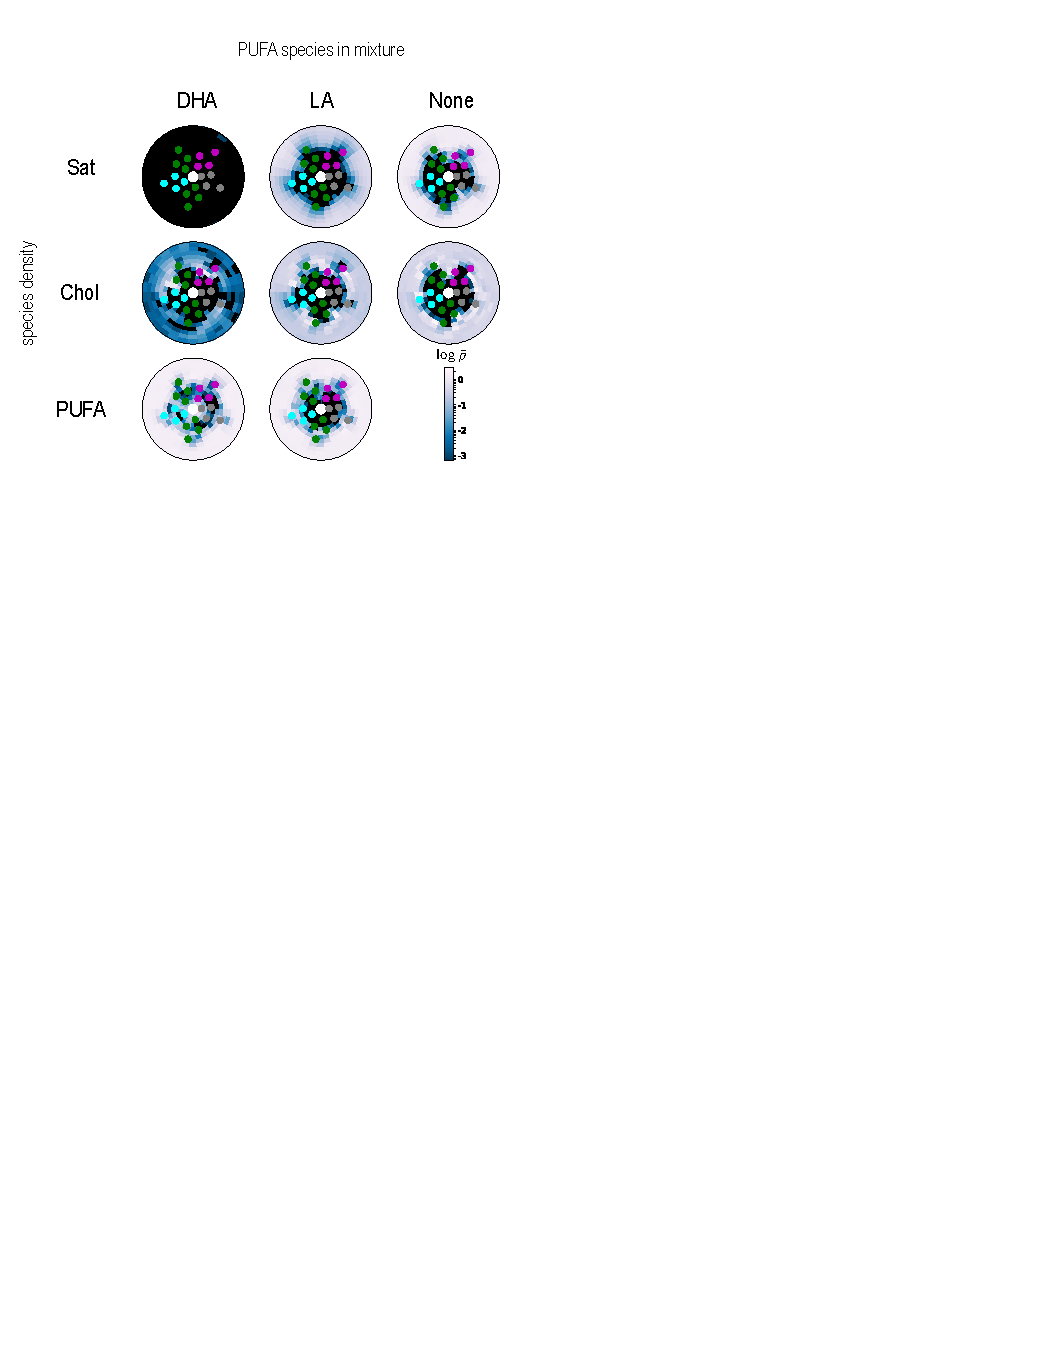
\includegraphics[width=\linewidth,trim={0cm 0cm 0cm 0cm}]{Fig3}
\caption[Pairwise distance distribution across multi-protein systems.] {{\bf Radial distribution function g(r)  of pairwise protein center-of-mass distances, across multi-protein systems.}  Data collection began at 2 $\mu s$ into each trajectory and ended at 10 $\mu s$, respectively. The peak between 7-10 nm corresponds to dimer formation.  }
\label{fig:Figure6}
\end{figure}

%In Figure ~\ref{fig:Figure5}, three subplots depict the average distance between pairs of distinct proteins, in systems containing two, three, or four nAChRs. Across 1500-4000 ns trajectories, the average distance between distinct pairs of proteins is smaller in membranes with well-defined domains, compared to those lacking domains. 

%In the majority of domain-forming membranes, twe observed the formation of nAChR dimers along domain interfaces. Along domains, a majority of pairwise distances  fell within 100-150 {\AA} by 3000 ns (see Figure \ref{fig:Figure4}). This trend persisted within and across individual simulations, regardless of protein concentration or the size and shape of domains.

%\begin{figure}[H]
%	\center
%	\includegraphics[width=\linewidth]{Figure5}
%\caption[Average pairwise distance between nAChR molecules over time.] {{\bf Average pairwise distance between nAChR molecules over time.} Pairwise distance vs time for 12 multi-protein systems.  Here pairwise distance is the average distance between the centers of mass across pairs of proteins.}
%\label{fig:Figure5}
%\end{figure}


\subsection{Closest subunits across dimerizing proteins}
In order to determine whether nAChR dimers were more likely to form with specific subunit interactions, we determined the closest interacting subunit pair for nAChR dimers within each frame. To ensure that dimers, rather than larger oligomers, were being analyzed, we excluded trimers and tetramers from the analysis and only considered two protein systems, with increased sampling. Figure ~\ref{fig:Figure7} shows the amount of enrichment for each possible subunit pairing, relative to an expected random distribution. Results were very sensitive to the use of domain-forming compositions. In heteroacidic membranes, the $\alpha_{\delta}$ subunit formed a monomer-monomer interaction with the $\beta$ subunit, while the $\alpha_{\gamma}$ most favorably interacted with the $\delta$ subunit. In domain-forming membranes,  the $\delta-\alpha_{\delta}-\gamma$ interface was two to five times as likely to pair with a $\alpha_{\delta}$ subunit compared to a random distribution, but substantially more dispersion was detected than in non-domain forming membranes. This difference suggests that nAChRs have preferred dimerization orientations, but membrane organization can reorient receptors. Although $\delta$ subunits are linked by a disulfide bond at the NMJ \citep{Chang1977}, our simulations suggest that without this link, $\delta$ subunits do not form the closest pair among dimerizing proteins.

%{If we do not use three and four protein systems in figure 7, would it be appropriate to discuss possible subunit-subunit pairing for greater number of proteins? Looking at the current plots, I am ''expecting'' if we added more proteins, they would begin to pair off along the white blocks.. }
%Liam, I commented out your remark because GB already addressed it on paper.
%     formation  dependent on  the nAChR $\alpha_{\delta}$ subunit most frequently formed the closest pair, pairing with $\delta$, and $\gamma$ subunits well above expectation (10-15 \%) in both domain-forming and hybrid membranes. In domain-forming membranes, the most frequent closest subunit pairs were $(\alpha_\delta, \delta)$ and $(\alpha_\delta, \gamma)$, each appearing in more than 15 \% of simulations. In hybrid membranes, in addition to the $\alpha_{\delta}$ subunits mentioned above, $(\alpha_\gamma, \gamma)$ were among the closest subunits at a level above expectation. On the other hand, the nAChR $\beta$ subunits formed the fewest subunit pairs, falling well below the expectation value for each pair. Please refer to Figure ~\ref{fig:Figure7} for a heat-map of these data.   



\begin{figure}[htp]
	\center
	\includegraphics[height=3in]{images/Fig4_new}
\caption[Subunit pairs among dimerizing proteins]{{\bf Most probable subunit pairs among dimerizing proteins.} Heat-map showing the likelihood that two subunits were closest together among dimerizing proteins (100 {\AA} threshold). Distinct subunits are each expected to form the closest pair 8 \% of the time, while identical subunits are each expected to dimerize only 4 \% of the time. Each color on the heatmap represents multiplicative depletion or enrichment relative to the pair's expectation value, ranging from complete depletion (red) to no enrichment (white) to five-fold enrichment (blue).  }
\label{fig:Figure7}
\end{figure}

\section{Discussion} 

%{nAChR's native membranes, \textit{Torpedo} and synapses, are rich in the n-3 PUFA, DHA. DHA, along with other PUFAs have been shown to improve cognitive functioning, cardiac health, and various diseases.}
%Found primarily in fish oil, polyunsaturated fatty acids have been generally associated with enhanced cognitive functioning, as well as benefits in cardiac health and disease prevention 
%\citep{12439486320170901}.
%As stated previously, 

The nAChR is one of the most well-studied, fundamental pLGICs for understanding human cognition, memory, and muscle contraction \citep{Gotti1997}. As an integral membrane protein, the function and organization of nAChR is strongly dictated by its surrounding lipid environment. DHA is an $\omega$-3 polyunsaturated fatty acid abundant in synaptic membranes and the Torpedo electric organs, which are both native nAChR membranes. With its six double bonds, DHA is considered highly disordered and can induce domain formation in membranes \citep{S000930840800032720080101}. We previously observed \citep{Sharp2019} favorable interactions between a single nAChR and DHA-rich, cholesterol-poor domains using coarse-grained simulations. Here, we have extended this approach to investigate the role of lipid topology and domain-formation on boundary lipids of individual nAChRs. We have also conducted the first simulations containing multiple nAChRs, which has allowed us to observe spontaneous dimerization.  

While DHA is implicated in human health and disease, \citep{12439486320170901} experimental studies considering its interactions with nAChR have exclusively considered its free-fatty acid form (FFA), \citep{Antollini2016} %https://www.frontiersin.org/articles/10.3389/fphys.2016.00573/full#h3
rather than as an acyl chain component of a phospholipid. Application of $\omega-3$ FFAs causes a significant reduction in open times observed through single-channel recordings  \citep{Bouzat1993}. Here, we observe a substantial effect of lipid topology on both embedded and annular lipids: DHA chains in homoacidic phospholipids are far more likely to be found as either annular or embedded boundary lipids.  We previously observed only quantitative effects of swapping PE with PC on partitioning, but the headgroup does serve to anchor the lipid at the membrane/protein interface  \citep{Sharp2019}.  DHA in its FFA form (without a headgroup) may diffuse into an open nAChR pore, blocking the channel. %https://www.ncbi.nlm.nih.gov/pubmed?Db=pubmed&Cmd=ShowDetailView&TermToSearch=7522903

We find that, consistent with coarse-grained MD simulations using one nAChR \citep{Sharp2019}, multiple nAChRs continue to prefer the liquid-disordered phase containing long-chain $\omega$-3 fatty acids. While the number of nAChRs in the system did not affect the partitioning profile in these simulations, it did affect the composition of embedded lipids. Our results are consistent with each nAChR monomer in an oligomer blocking access to embedded lipid binding sites in the other monomers, suggesting an intriguing coupling between specific binding and membrane organization.  

Interestingly, upon removing membrane organization, embedded lipids cluster around specific transmembrane helices in a five-fold symmetry around nAChR. This finding suggests that intrinsic lipid preferences are primarily helix dependent, rather than subunit dependent. In homoacid membranes, a lipid preference for DHA was observed across all transmembrane helices, with shells of PUFAs found even at the border of the liquid-ordered phase. Although saturated acyl chains and cholesterol were generally depleted around nAChR, the highest densities for both lipids were found around the M1 and M3 helices, as seen in heteroacid membranes.

In native membranes, nAChR dimers can be stabilized by a disulfide bond between $\delta$ subunits \citep{Chang1977}.  An early controversy \citep{Anholt1980,Ruechel1981,Zingsheim1982,Schindler1984} concerned whether the disulfide bond was necessary for dimer formation. There is no mechanism for covalent bonds between monomers in these coarse-grained simulations. All dimers were stabilized by non-covalent interactions, consistent with the results of \citep{Ruechel1981,Schindler1984}. We observed far more stable dimers in the homoacid mixtures than the heteroacid mixtures, which would be consistent with high sensitivity to experimental conditions. We did not observe a consistent $\delta-\delta$ preference for interfacing subunits in either homoacid or heteroacid mixtures. Schindler {\it et al} (1984) observed an apparent gain-of-function for single-channels within dimers relative to monomers, regardless of disulfide linking \citep{Schindler1984}, suggesting that lipid modulation of oligomerization could also provide a pathway for modulating single channel function. 
%More specifically, nAChRs partitioned into DHA-enriched domains. 
%%
%%%%
%%
%%%While it is well-established that cholesterol leads to a gain-of-function in nAChR, adding anionic lipids like POPA to a purely POPC or POPC:CHOL reconstitution mixture also results in significant gain-of-function, causing some researchers to suggest anionic lipids are required for functional conformations of nAChR \citep{Corrie_Lipid_2002}. If so, we might expect anionic lipids (such as the DHA-PS used here) to have a higher probability of being in the nAChR boundary than zwitterionic lipids. Instead, we find that anionic lipids and zwitterionic lipids (PE headgroups) had similar affinities for nAChR's TMD. It is important to emphasize that in domain-forming membranes, PS and PE phospholipids both had DHA acyl chains and their probabilities of embedding were much higher compared to those in hybrid mixtures (See Figure \ref{fig:Figure3}). While cholesterol embedded throughout the nAChR transmembrane bundle, DHA-PS and DHA-PE occupied these non-annular sites in higher concentrations. This supports the hypothesis that, alongside cholesterol, PUFAs can provide additional support to nAChR structural and functional integrity, as hypothesized by Sharp et. al (2018) \citep{Sharp2018}.
%%
%%
%%To our knowledge, previous studies have not included PUFAs in their membrane mixtures, which may affect the interactions between lipids and the nAChR ion pore. \citep{Fong_Correlation_1986,Sunshine_Lipid_1992,Butler1993,Fong_Stabilization_1987,Corrie_Lipid_2002}. Our data show that by inducing domain formation in membranes, DHA leads to the clustering of nAChRs in the flexible, liquid-disordered phase and supports their boundary acyl chain preference for PUFAs (Figure \ref{fig:Figure3}). Without domain formation, since hybrid lipids only have one DHA chain each, DHA cannot aggregate around nAChRs to the same degree. 
%%
%%
%%%Additionally, by clustering along specific nAChR subunits, neuromuscular nAChRs  may also depend on protein sequence for the early stages of nAChR dimerization. 
%%Pentameric ligand-gated ion channels, such as nAChR and GABA-A, have retained function for millions of years and are found in many species - from bacteria to humans; however, heteromers, which include $\gamma$ or $\delta$ subunits, are found in higher-level organisms and between synapses \citep{Jaiteh2016}. In our simulations, $\delta$ and $\gamma$ subunits promoted oligomerization of muscle-type nAChRs. This preference in subunit pairs may indicate an essential role for heteromerization in pLGIC oligomerization within the nervous system. Building on this work, we aim to expand the scope of our computational models, with special consideration to the individual effects of membrane elasticity, protein concentration, and pLGIC sequence on nAChR oligomerization.  







% For one-column wide figures use
%\begin{figure}
% Use the relevant command to insert your figure file.
% For example, with the graphicx package use
%  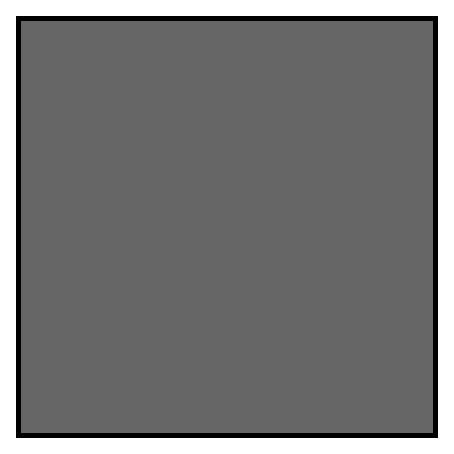
\includegraphics{example.eps}
% figure caption is below the figure \caption{Please write your figure caption here}
%\label{fig:1}       % Give a unique label
%\end{figure}
%
% For two-column wide figures use
%\begin{figure*}
% Use the relevant command to insert your figure file.
% For example, with the graphicx package use
 % 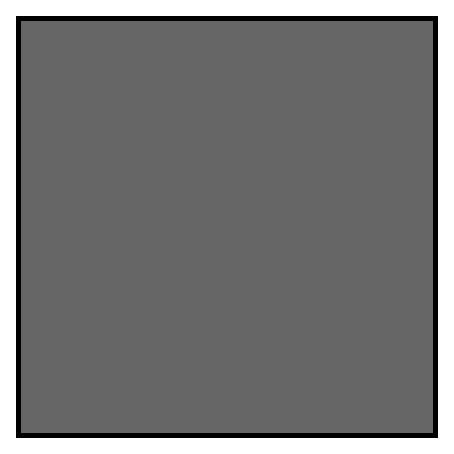
\includegraphics[width=0.75\textwidth]{example.eps}
% figure caption is below the figure
%\caption{Please write your figure caption here}
%\label{fig:2}       % Give a unique label
%\end{figure*}; however, both of these interactions were considered weak. Overall, heteroacid mixtures closely matched a probability distribution of random subunit pairing.
%
% For tables use
%\begin{table}
% table caption is above the table
%\caption{Please write your table caption here}
%\label{tab:1}       % Give a unique label
% For LaTeX tables use
%\begin{tabular}{lll}
%\hline\noalign{\smallskip}
%first & second & third  \\
%\noalign{\smallskip}\hline\noalign{\smallskip}
%number & number & number \\
%number & number & number \\
%\noalign{\smallskip}\hline
%\end{tabular}
%\end{table}
%

\begin{acknowledgements}
GB was supported by research grants NSF MCB1330728 and NIH P01GM55876-14A1. GB and LM were also supported through a grant from the Research Corporation for Scientific Advancement. This project was supported with computational resources from the National Science Foundation XSEDE program through allocation NSF-MCB110149, a local cluster funded by NSF-DBI1126052, the Rutgers University Office of Advanced Research Computing (OARC) and the Rutgers Discovery Informatics Institute (RDI2), which is supported by Rutgers and the State of New Jersey. We are grateful to Dr. J\'{e}r\^{o}me H\'{e}nin for his helpful suggestions throughout this study.  
\end{acknowledgements}

% BibTeX users please use one of
%\bibliographystyle{spbasic}      % basic style, author-year citations
%\bibliographystyle{spmpsci}      % mathematics and physical sciences
%\bibliographystyle{spphys}       % APS-like style for physics
%\bibliography{}   % name your BibTeX data base  

% Non-BibTeX users please use
%\begin{thebibliography}{}
%
% and use \bibitem to create references. Consult the Instructions
% for authors for reference list style.
%

\section{Compliance with Ethical Standards}
{\bf Conflict of interest:} The authors declare that they have no conflict of interest. This research was supported in part by the National Science Foundation, the National Institutes of Health, and the Research Corporation for Scientific Advancement. 

%\bibitem{RefJ}
% Format for Journal Reference
\bibliographystyle{spbasic}
\bibliography{BIBx.bib}
%\end{thebibliography}

\end{document}
% end of file template.tex
